\section*{Problem Sheet 1: Relativistic Kinematics}
\label{sec:ps1}
\newcounter{psOneQuestions}
\setcounter{psOneQuestions}{0}
\newcommand{\NewQuestion}[1]{\stepcounter{psOneQuestions}\subsection*{Exercise \arabic{psOneQuestions}: #1}}

\NewQuestion{
This question is about Feynman diagrams in QED. To answer this you can follow the solved example in your notes.}
\begin{enumerate}[(i)]
\item Draw a Feynman diagram for each of the  QED processes $e^+e^-\to \mu^+\mu^-$ and $e^+e^-\to q\bar{q}$ clearly labelling the vertex factors of the processes. The symbols  $q$ and $\bar{q}$ denote a quark and anti-quark with electric charge $\pm e_q$. 
\item By assuming that the Centre-Of-Mass energy of both processes are the same and ignoring the masses of all the particles involved, show that the matrix elements squared of the two processes are related by \[
\left |\frac{\mathcal{M}_{\mu\mu}}{\mathcal{M}_{q\bar{q}}}\right |^{2} = \frac{e^2}{e_{q}^{2}}
\]
\item What is the physical meaning of $|\mathcal{M}_{\mu\mu}|^{2}$ and $|\mathcal{M}_{q\bar{q}}|^{2}$ 
\end{enumerate}
\answerbox{
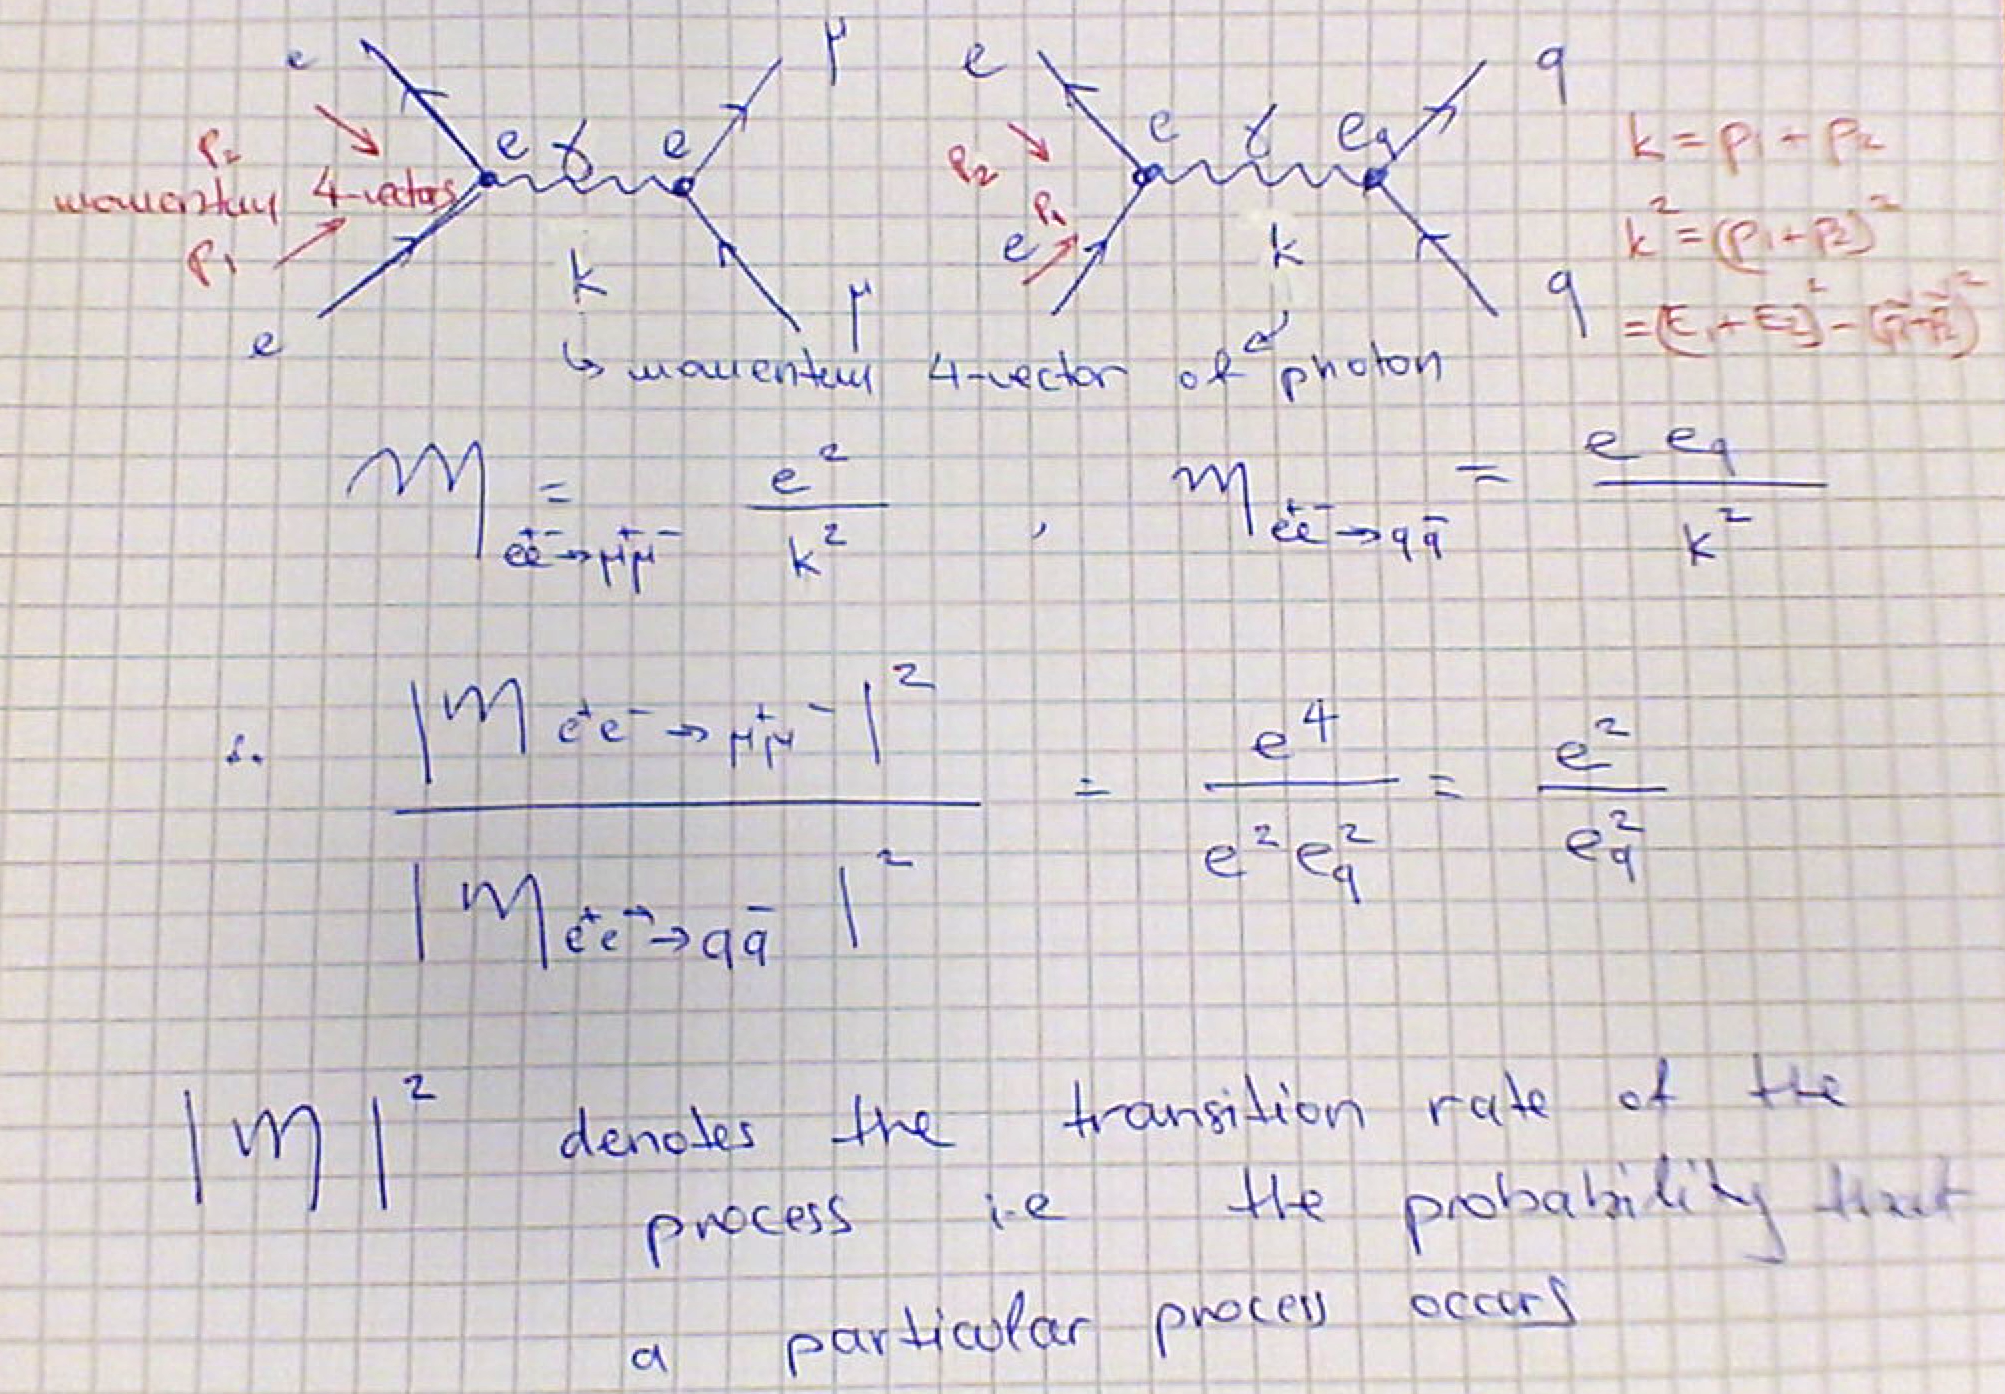
\includegraphics[width=0.9\textwidth]{problemsheets/ps1figs/ps1_q1_ans.png}
}

\NewQuestion{This question is about basic 4-vector manipulation}
You are given two 4-vectors
\[U=(u_0,\vec{u})\] and
\[Y=(y_0,\vec{y})\]
You are given that the opening angle between $\vec{u}$ and $\vec{y}$ is $\theta$. 
Write down an expression of $U\cdot Y$ in terms of $\theta$, $u_0$, $y_0$, $|\vec{u}|$ and $|\vec{y}|$.
\answerbox{
Following the definition of 4-vector dot products
\[
U\cdot Y= u_0y_0-\vec{u}\cdot\vec{y}
\]
Following the definition of 3-vector dot products
\[
U\cdot Y= u_0y_0-|\vec{u}||\vec{y}|cos\theta
\]
}

\NewQuestion{This question is about basic 4-vector Lorentz Transformations}
You are given two 4-vectors in frame $S$.
\[U=(u_0,\vec{u})\] and
\[Y=(y_0,\vec{y})\]
 Lets now consider a frame $S'$ moving with constant velocity along the $x$ direction with $\beta=v/c$. 
 By considering how the various components of $U$ and $Y$ transform under a Lorentz Transformation along the $x$-axis, show that the quantity $U\cdot Y$ is invariant under this transformation
\answerbox{
\[U^{'}\cdot Y^{'}=U_{0}^{'}Y_{0}^{'}-U_{x}^{'}Y_{x}^{'}-U_{y}^{'}Y_{y}^{'}-U_{z}^{'}Y_{z}^{'}
\]
But boost only along the $x$ axis so 
\[
U_{0}^{'}=\gamma U_0-\beta\gamma U_x,\\
U_{x}^{'}=-\beta\gamma U_0+\gamma U_x,\\
U_{y}^{'}=U_{y},\\
U_{z}^{'}=U_{z}
\]

So inserting into equation we have
\begin{equation*}
\begin{split}
U^{'}\cdot Y^{'}&=\gamma^2U_0Y_0(1-\beta^2)-     \\ &\quad\gamma^2U_xY_x(1-\beta^2)-\gamma^2\beta U_0Y_x- \\ 
&\gamma^2\beta U_xY_0+\beta^2\gamma^2U_xY_x+\beta\gamma^2U_0Y_x+\\
&\beta\gamma^2U_xY_0-U_{y}Y_{y}-U_{z}Y_{z}
\end{split}
\end{equation*}
Remembering that $\gamma^2=\frac{1}{1-\beta^2}$ and cancelling common terms
\[
U^{'}\cdot Y^{'}=U_0Y_0-U_xY_x-U_yY_y-U_{z}Y_{z}
\]

}

\NewQuestion{This question is about relativistic  kinematics}

Show that the energy momentum relationship
\[ E^2=p^2c^2+m^2c^4\] follows from the expressions $E=\gamma m c^2$ and $p=\gamma mv$ 
Hint: start from  $\gamma=\frac{1}{\sqrt{1-v^2/c^2}}$ and solve for $v$. Then insert this expression for v into $p=\gamma mv$
\answerbox{Start by using the expression of $\gamma$ to solve for $v$ and get 
\[v=\sqrt{(\gamma^2-1)}c/\gamma\]
Inserting this expression into $p=\gamma mv$ we have that \[p=mc\sqrt{\gamma^2-1}\] and thus
\[\gamma=\sqrt{p^2/(m^2c^2)+1}\]. Inserting this into $E=\gamma mc$ we have that
\[
E^2=(p^2/(m^2c^2)+1)m^2c^4
\]
and thus
\[
E^2=p^2c^2+m^2c^4
\]
}

\NewQuestion{This question is about applying relativistic particle kinematics to various particle collider examples}

What are the Centre of Mass energies of the following particle accelerator facilities?
\begin{enumerate}[(i)]
\item LEP1: $e^+e^-$ collider both beams at 45.6~GeV. \\If we wanted to produce a $Z^0$-boson of mass 91.2~GeV$/c^2$ AND a Higgs-boson of mass 125~GeV$/c^2$ simultaneously from an $e^+e^-$ collision, what is the minimum centre of mass energy required?
\item LHC: $pp$ collider both beams at 7~TeV
\item HERA: $ep$ collider $E_e=30$~GeV and $E_p=920$~GeV. If HERA was to collide instead electrons onto protons of a stationary target, what would the required electron beam energy be in order to achieve the same centre of mass energy?
\end{enumerate}
You can assume $m_e=0.5$~MeV$/c^2$ and $m_p=1$~GeV$/c^2$.
\answerbox{

For colliders where the beam energies are equal (ie cases (i) and (ii))

$\vec{p}_{1}+\vec{p}_{2}=0$. That means that given the definition of the centre-of-mass energy
\[
\sqrt{s}=\sqrt{(E_1+E_2)^2-(\vec{p}_1+\vec{p}_2)^2}=E_1+E_2
\]
Therefore for \\
(i) $\sqrt{s}=2\times 45.6=91.2$GeV\\
The minimum energy required required to produce a Higgs-boson of mass 125GeV/$c^2$ corresponds to the case when the Higgs-boson and the $Z^0$ are produced at rest. Therefore the minimum energy required would be equal to the rest-energy of the Higgs and $Z^0$ combined, ie $\sqrt{s}_{min}=m_{H}c^2+m_{Z^0}c^2=91.2+125$GeV

(ii) $\sqrt{s}=2\times 7=14$TeV\\

(iii) Here $E_e=30$GeV and $E_p=920$GeV. Therefore $|p_e|=\sqrt{E_e^2-m_e^2}\sim E_e=30$GeV. Similarly,  $|p_p|=\sqrt{E_p^2-m_p^2}\sim E_p=920$GeV.
So
\begin{equation*}
\begin{split}
\sqrt{s}=&\sqrt{(E_e+E_p)^2-(\vec{p}_e+\vec{p}_p)^2}\\
=& \sqrt{E_{e}^{2}+E_{p}^{2}+2E_eE_p-|\vec{p}_e|^{2}-|\vec{p}_p|^{2}-2\vec{p}_e\vec{p}_pcos\pi}
\end{split}
\end{equation*}

where we have taken the angle between the two beams as $\pi$ as they are colliding head on. Given we can approximate $E$ with $|p|$ as the beam energies are much larger than rest masses we have
\[
\sqrt{s}\sim\sqrt{4E_eE_p}\sim332\mathrm{GeV}
\]

Now for a fixed target configuration, from our notes we have that 
\[
E_e\sim \frac{s}{2m_p}
\]
for the case when $\sqrt{s}\gg m_e,m_p$ which is indeed the case in this problem.
Therefore $E_e\sim 55$TeV in order to reach $\sqrt{s}=332$GeV in a fixed target configuration

}


\NewQuestion{This question is about relativistic kinematics}
A $B^0$ meson is a bound state between an anti-$b$ and a $d$ quark and has a mass of $5.28$~GeV$/c^2$. The average time before the $B^0$ decays (ie its mean life-time) is 1.5~ps (1~ps=1$\times 10^{-12}$~s). Given that the average momentum of the $B^0$ meson as measured by the ``LHC beauty'' (LHCb) experiment is 100~GeV$/c$, calculate the average distance it travels before it decays, as measured by the experimenters.
\answerbox{
Average momentum of the $B^0$ is given by
\[
<|\vec{p}_{B}|>=\gamma m_B<v_B>
\]
And average displacement is
\[
<d_B>=<v_B>t_B
\]
Where $t_B$ is the lifetime in the lab frame. However $t_B=\gamma\tau_B$ where $\tau_B$ is the average lifetime of the $B$ in its rest frame (proper lifetime).
Therefore using the expression of the average momentum above we have
\[
<d_B>=<|\vec{p}_{B}|>/m_B\times \tau_B = \frac{100{\rm GeV/c}}{5.28{\rm GeV/c^2}}\times1.5\times10^{-12}{\rm s}
\]
Thus $<d_B>=\frac{100}{5.28}c1.5\times10^{-12}=0.0085$m
}




%%\NewQuestion{
%%{\bf Do at home! An interesting question but not %%examinable}
%%This question walks you through the proof that the %%Klein-Gordon equation is problematic as
%%suggests that the probability density of a %%wave-function $\psi(x)$ can be negative 
%%}
%%\begin{enumerate}[(i)]
%%\item Show that a wave-function of the form
%%\[
%%\psi=Ne^{i(\vec{p}\cdot\vec{x}/\hbar-E/\hbar t)}
%%\]
%%where $N$ is a complex proportionality constant, is a %%solution to the Klein-Gordon equation:
%%\[
%%(\frac{1}{c^2}\frac{\partial^{2}}{\partial %%t^2}-\vec{\nabla}^2)\psi+\frac{m^2c^2}{\hbar^2}\psi=0
%%\]
%%with energy states given by:
%%\[
%%E=\pm\sqrt{p^2c^2+m^2c^4}
%%\]
%%
%%\item The continuity equation is given by:
%%\[
%%\frac{\partial\rho}{\partial %%t}+\vec{\nabla}\vec{j}=0,
%%\]
%%where $\rho$ represents a quantity per unit volume  %%(e.q charge density) and $j$ is the flux of that %%quantity (e.g current per unit area flowing through a %%surface).
%%In quantum mechanics the continuity equation %%expresses the flow of probability in complete analogy %%to electromagnetism or fluid mechanics. The flux in %%this case is the probability per unit time per unit %%area that the particle will pass through a surface. %%The continuity equation in quantum mechanics reflects %%the fact that a particle moves through space in a %%continuous manner and that the integral of  the %%probability distribution of its position over all %%space is always 1.
%%
%%By rewriting the Klein-Gordon equation to look like %%the continuity equation  show that the probability %%density $\rho$ and $\vec{j}$ can be given by 
%%\[
%%\rho=i(\psi^*\frac{\partial \psi}{\partial %%t}-\psi\frac{\partial \psi^*}{\partial t})
%%\]
%%and 
%%\[
%%\vec{j}=ic^2(\psi\vec{\nabla}\psi^*-\psi^*\vec{\nabla%%}\psi)
%%\]
%%\item Subsequently show that:
%%\[
%%\rho=\pm 2\sqrt{p^2+m^2}|N|^2.
%%\]
%%Hint: take complex conjugate of %%Eq.~\ref{eq:klein_gordon} and  multiply both left and %%right-hand side by $\psi$). Also multiply both left %%and right-hand side of Eq.~\ref{eq:klein_gordon} by %%$\psi^*$.
%%\end{enumerate}
%%\answerbox{}

